
    \documentclass{article}
    \usepackage[a4paper, left=2cm, right=2cm, top=1cm, bottom=2cm]{geometry}
    \usepackage{amsmath}
    \usepackage{graphicx}
    \begin{document}

    \begin{figure}[h!]
        \centering
        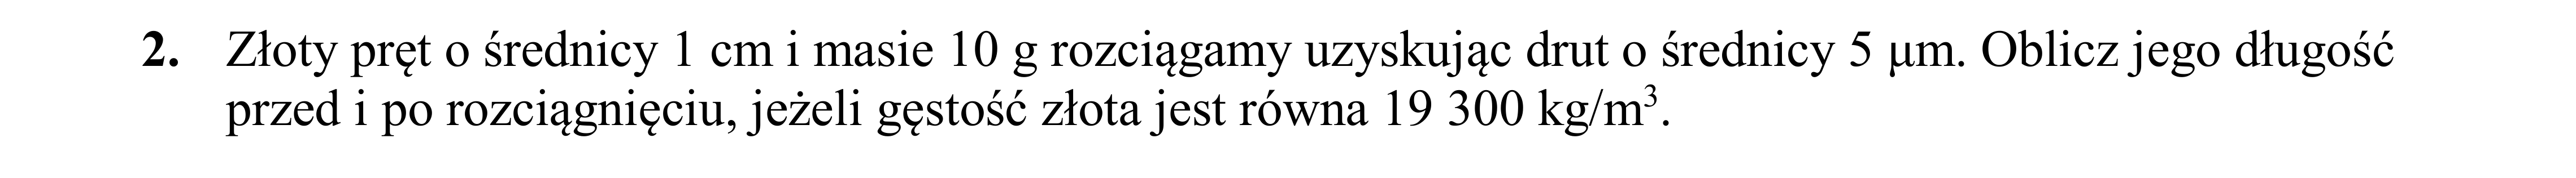
\includegraphics[width=1\textwidth]{Solutions/Zestaw 01/desc_02.png}
    \end{figure}

    \begin{quote}
    Aby rozwiązać zadanie, najpierw ustalmy dane:

- Masa złotego pręta \( (m) = 10 \, g = 0.01 \, kg \)
- Średnica pręta \( (d_1) = 1 \, cm = 0.01 \, m \)
- Gęstość złota \( (\rho) = 19300 \, kg/m^3 \)

### Kroki do rozwiązania:

1. **Oblicz objętość złotego pręta:**

   Gdy mamy masę i gęstość, możemy obliczyć objętość \( V \):

   \[
   V = \frac{m}{\rho}
   \]

   \[
   V = \frac{0.01 \, kg}{19300 \, kg/m^3} \approx 5.18 \times 10^{-7} \, m^3
   \]

2. **Oblicz długość pręta przed rozciągnięciem:**

   Obliczamy pole przekroju poprzecznego pręta:

   \[
   r_1 = \frac{d_1}{2} = 0.005 \, m
   \]

   \[
   A = \pi r_1^2 = \pi (0.005)^2 \approx 7.85 \times 10^{-5} \, m^2
   \]

   Użyjemy wzoru na objętość walca, aby obliczyć długość \( L_1 \):

   \[
   V = A \cdot L_1 \implies L_1 = \frac{V}{A}
   \]

   \[
   L_1 = \frac{5.18 \times 10^{-7} \, m^3}{7.85 \times 10^{-5} \, m^2} \approx 0.0066 \, m = 6.6 \, mm
   \]

3. **Oblicz długość drutu po rozciągnięciu:**

   Średnica nowego drutu \( (d_2) = 5 \, \mu m = 5 \times 10^{-6} \, m \)

   Obliczamy jego pole przekroju poprzecznego:

   \[
   r_2 = \frac{d_2}{2} = 2.5 \times 10^{-6} \, m
   \]

   \[
   A_2 = \pi r_2^2 = \pi (2.5 \times 10^{-6})^2 \approx 1.96 \times 10^{-11} \, m^2
   \]

   Używamy objętości drutu do obliczenia długości \( L_2 \):

   \[
   L_2 = \frac{V}{A_2}
   \]

   \[
   L_2 = \frac{5.18 \times 10^{-7} \, m^3}{1.96 \times 10^{-11} \, m^2} \approx 26461.22 \, m
   \]

### Ostateczny wynik:
Długość drutu o średnicy 5 μm wynosi około \( 26461.22 \, m \) (czyli 26.5 km).
    \end{quote}
    \end{document}
    